\documentclass{article}

\usepackage[T1]{fontenc}
\usepackage{amsmath}
\usepackage{amssymb}
\usepackage{mathtools}
\usepackage{algpseudocode}
\usepackage[inline]{enumitem}
\usepackage{listings}
\usepackage[framed]{matlab-prettifier}
\usepackage{pgfplots}
\usepackage[Polish]{babel}
\usepackage{float}

\DeclarePairedDelimiter{\norm}{\lVert}{\rVert}

\title{Sprawozdanie \\Metody numeryczne 2 \\\textbf{Temat 4, Zadanie nr 12}}
\date{4/12/2018}
\author{Mateusz Śliwakowski, F4}

\begin{document}
  \pagenumbering{gobble}
  \maketitle
 	  \newpage
  \pagenumbering{arabic}

\section{Treść zadania}
\paragraph{}
Wzory empiryczne. Baza: $1,x,y,x^2y^2$. Tablicowanie błędów w punktach pomiarowych oraz obliczanie błędu średniokwadratowego. Punkty pomiarowe wybieramy z prostokąta $[a,b]\times[c,d]$.
\section{Opis metody}
\paragraph{}
Dana jest baza funkcji: $1,x,y,x^2y^2$, nazwijmy je $g_1,g_2,g_3,g_4$. Za ich pomocą chcemy aproksymować daną funkcję $f$ funkcją $f^*=\sum_{j=1}^4a_jg_j$ w taki sposób, aby $H = \sum_{i=1}^N(f(x_i)-f^*(x_i))^2 \longrightarrow min$. Zadanie sprowadza się do znalezienia współczynników $a_1, a_2, a_3, a_4\in \mathbb{R}$. $N$ to liczba punktów pomiarowych. Najczęściej powyższej metody używa się, gdy do danych zebranych doświadczalnie chcemy jak najlepiej dopasować krzywą.
\paragraph{}
Chcemy znaleźć minimum lokalne funkcji $H$:
$$\frac{\partial H}{\partial a_k}(a_1,\dots,a_4)\sum_{i=1}^N2(f(x_i)-\sum_{j=1}^4a_jg_j(x_i))(0 - g_k(x_i)) = 0$$
$$-\sum_{i=1}^Nf(x_i)g_k(x_i)+\sum_{i=1}^N\sum_{j=1}^4a_jg_j(x_i)g_k(x_i)=0$$
$$\sum_{j=1}^4a_j\sum_{i=1}^Ng_j(x_i)g_k(x_i) = \sum_{i=1}^Nf(x_i)g_k(x_i)\text{, gdzie } k = 1,\dots,4$$
\paragraph{}
Otrzymaliśmy układ równań normalnych:
$$\sum_{j=1}^4a_j<g_j,g_k>=<f,g_k>\text{, gdzie }k=1,\dots,4$$
\paragraph{}
Układ ten można zapisać jako $Ga=d$, gdzie:
\begin{itemize}
\item $G$ jest macierzą Gramma ($G_{jk}=<g_j,g_k>,j,k=1,\dots,n$)
\item $a=\begin{bmatrix} a_1\\a_2\\a_3\\a_4\end{bmatrix}$
\item $d=\begin{bmatrix} d_1\\d_2\\d_3\\d_4\end{bmatrix}$, $d_k=<f,g_k>,k=1,\dots,4$
\end{itemize}
\paragraph{}
Macierz Grama można zapisać jako $G=M^TM$, gdzie
$$M = \begin{bmatrix}
g_1(x_1) & g_2(x_1) & g_3(x_1) & g_4(x_1)\\
g_1(x_2) & g_2(x_2) & g_3(x_2) & g_4(x_2)\\
\vdots & \vdots & \vdots & \vdots\\
g_1(x_n) & g_2(x_n) & g_3(x_n) & g_4(x_n)
\end{bmatrix}$$
A wektor $d=M^TF$, gdzie $F=\begin{bmatrix}f(x_1)\\f(x_2)\\\vdots\\f(x_n)\end{bmatrix}$.
\section{Warunki i założenia}
\begin{enumerate}
\item Punkty pomiarowe są generowane losowo z prostokąta $[a,b]\times[c,d]$.
\item Dane $a,b,c,d,n$ są podane prawidłowo.
\item $f$ jest ograniczona na danym obszarze.
\end{enumerate}
\section{Implementacja}
\paragraph{}
Funkcja realizująca założenia zadania to \textit{lsfApproximation}.
\begin{lstlisting}[style=Matlab-editor]
function [fApprox, tab, err] = lsfApproximation(f,n,a,b,c,d)
\end{lstlisting}
\vspace{4pt}
Parametry wejściowe:
\begin{itemize}
\item $f$ - uchwyt do aproksymowanej funkcji dwóch zmiennych,
\item $n$ - ilość punktów pomiarowych,
\item $a,b,c,d$ - liczby rzeczywiste, definiujące prostokąt $[a,b]\times[c,d]$.
\end{itemize}
Parametry wyjściowe:
\begin{itemize}
\item $fApprox$ - uchwyt wynikowej funkcji ($f^*$),
\item $tab$ - tablica wynikowa zawierająca w kolumnach kolejno: współrzędne x oraz y punktu, wartość funkcji aproksymowanej w tym punkcie, wartość funkcji wynikowej, błąd,
\item $err$ - wartość błędu średniokwadratowego.
\end{itemize}
\paragraph{}
W implementacji postępujemy zgodnie z algorytmem przedstawionym w punkcie \textit{Opis metody}. Najpierw definiujemy funkcje z bazy i losujemy punkty pomiarowe. Potem przechodzimy do wyznaczenia macierzy kolejno: $M$, $G$, $F$, $d$, $a$ korzystając z operatorów Matlaba. Na koniec wszystkie wyniki tablicujemy oraz obliczamy błąd średniokwadratowy. 
\section{Przykłady i wnioski}
\paragraph{}
Na potrzeby prezentacji przykładów posłużymy się pomocniczą funkcją \textit{presentResult}, która wyświetla funkcje aproksymowaną i wynikową na jednym wykresie oraz konstruuje tablicę wynikową w przystępnym formacie.
\subsection{Funkcja z bazy}
Rozpocznijmy od sprawdzenia aproksymacji dla funkcji z bazy.
\begin{lstlisting}[style=Matlab-editor]
f = @(x,y) -5 + 4.*x - 2.*y + 3.*y.*y.*y.*y.*x.*x.*x.*x;
presentResult(f,10,-2,2,-2,2);
\end{lstlisting}
Otrzymujemy wynik z dokładnością maszynową. Na wykresie funkcja aproksyowana i wynikowa pokrywają się.
\begin{figure}[H]
  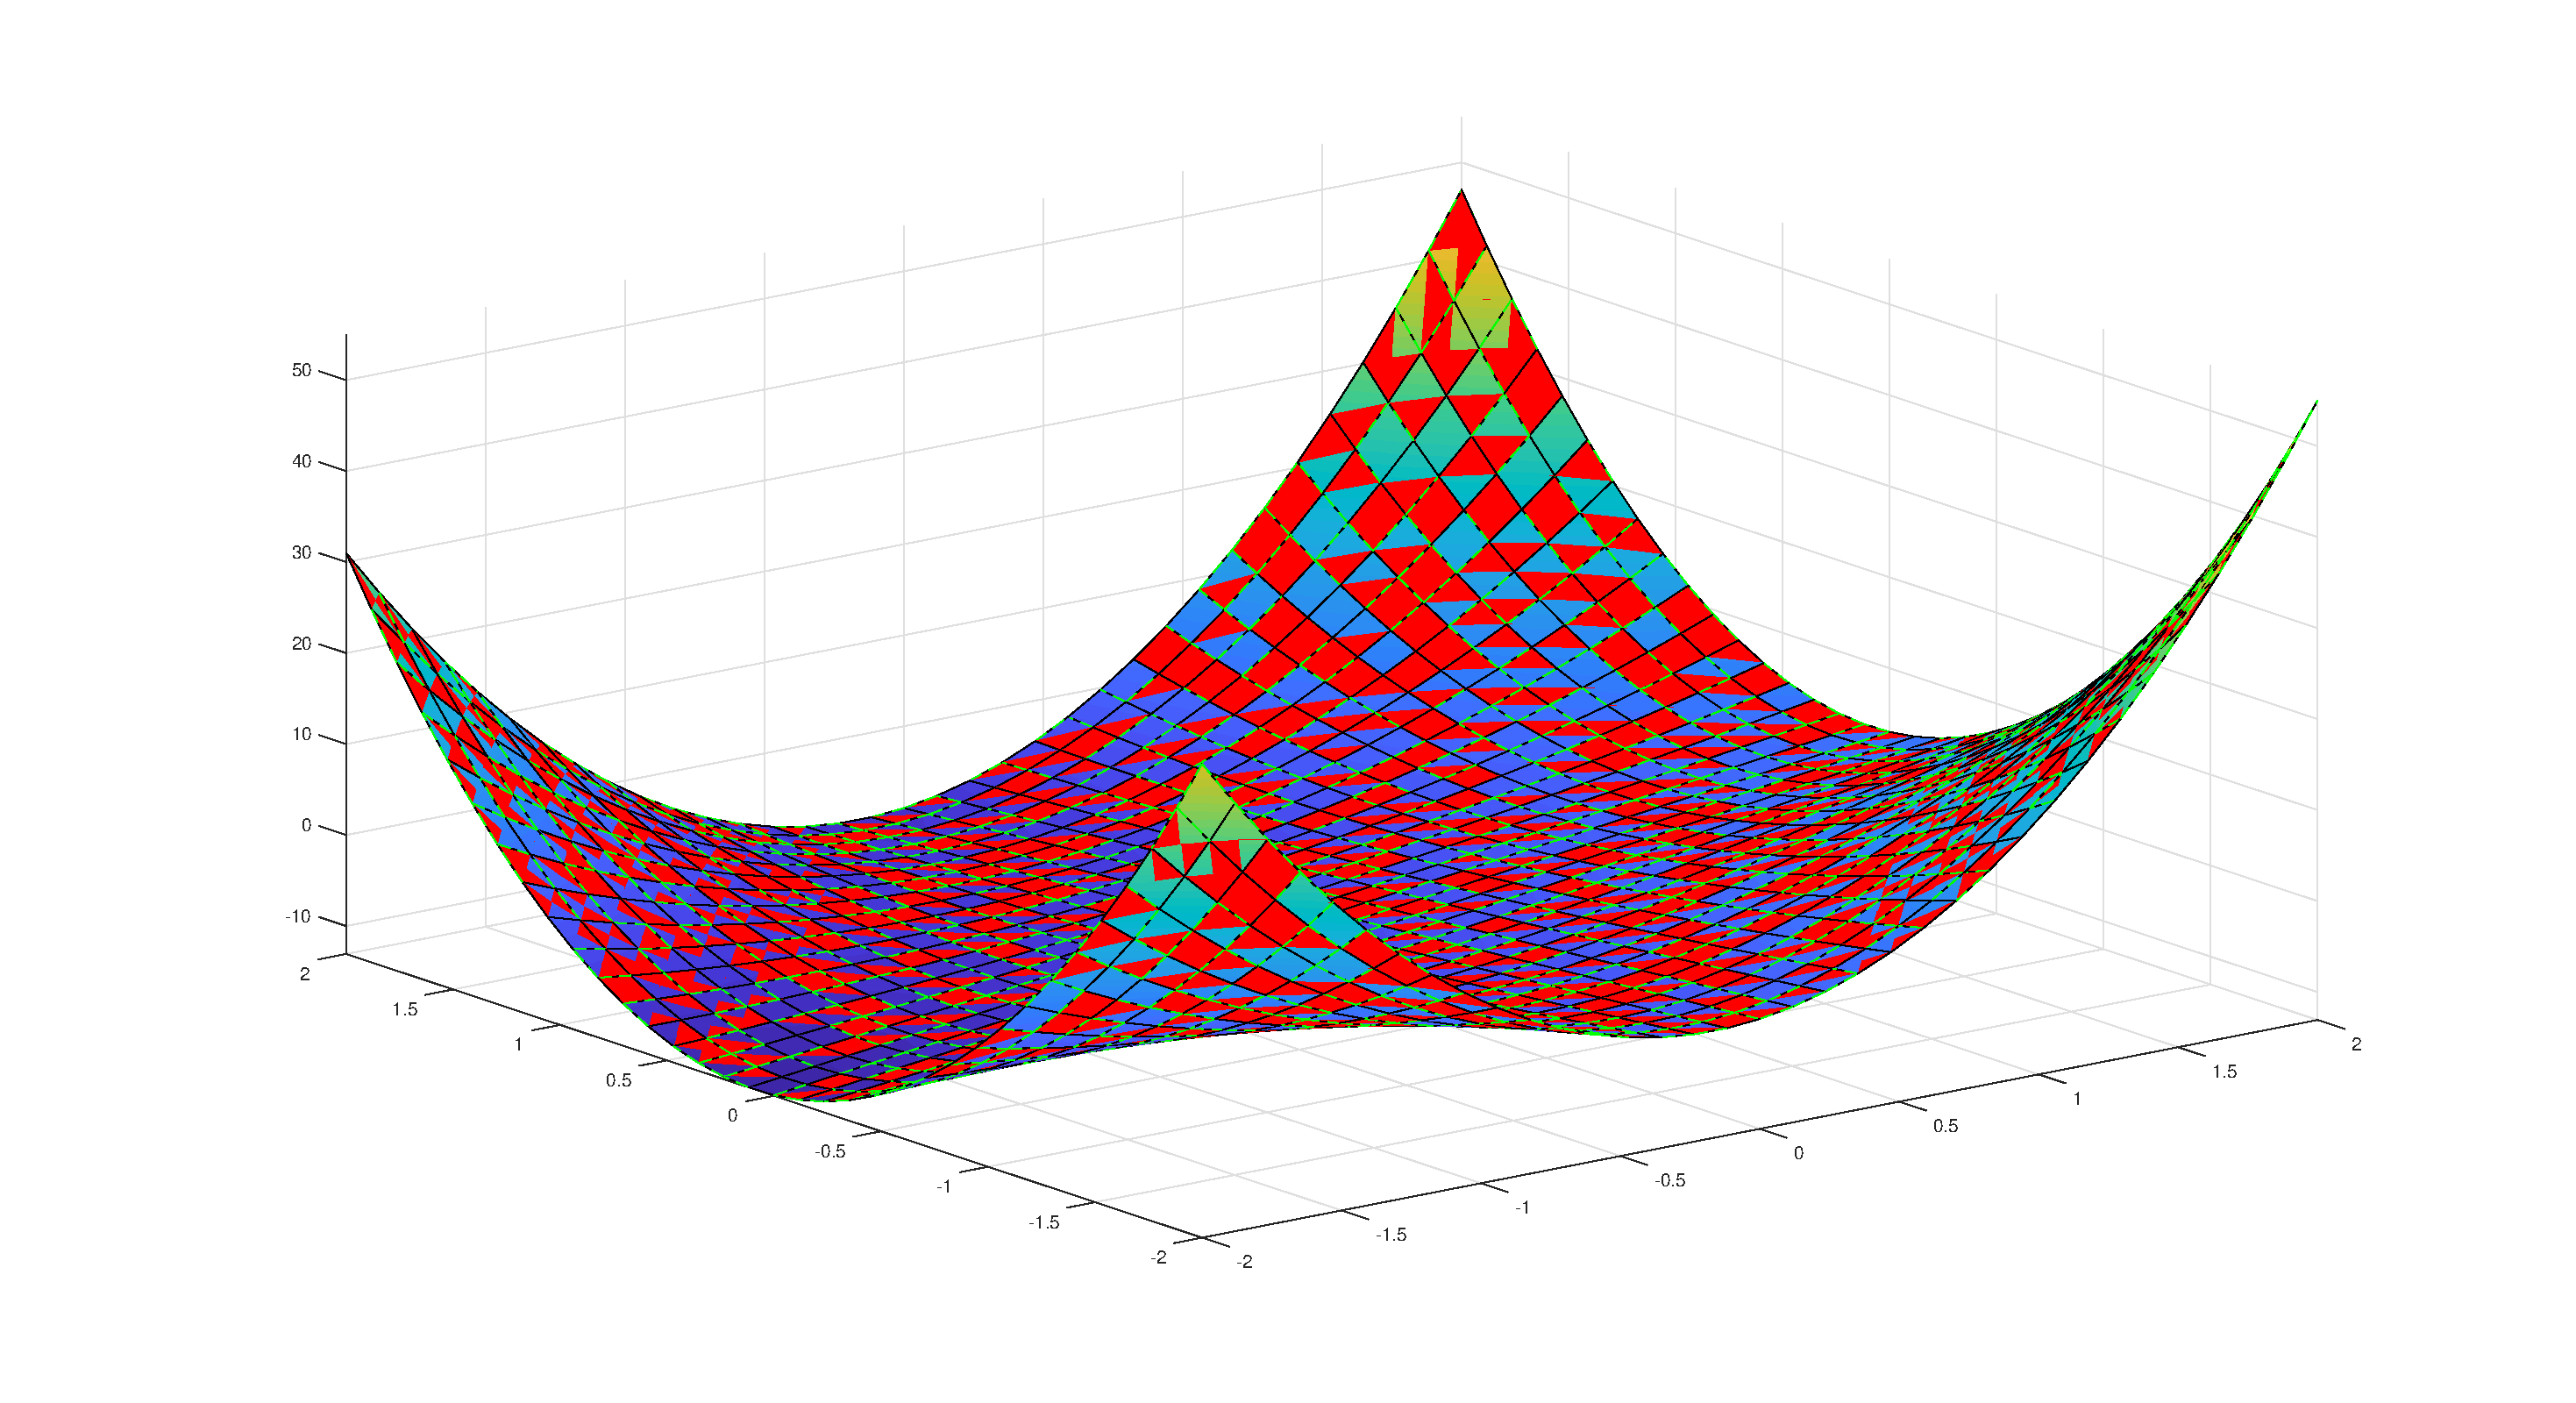
\includegraphics[width=\linewidth]{fig1.eps}
\end{figure}
Wartość błędu średniokwadratowego wynosi $2.0583e-15$. Porównywalne rezultaty otrzymujemy dla innych funkcji z bazy.
\subsection{Funkcja wielomianowa wyższego stopnia}
\paragraph{}
Następnie sprawdzimy działanie dla funkcji wielomianowej wyższego stopnia.
\begin{lstlisting}[style=Matlab-editor]
f = @(x,y) -5 + 4.*x - 2.*y + 3.*y.*y.*x.*x + 1.5.*x.*x.*x.*x.*y - 3.*y.*y.*y;
presentResult(f,10,-2,2,-2,2);
\end{lstlisting}
Kolorem czerwonym zaznaczona jest funkcja aproksymowana, zielonym - wynikowa.
\begin{figure}[H]
  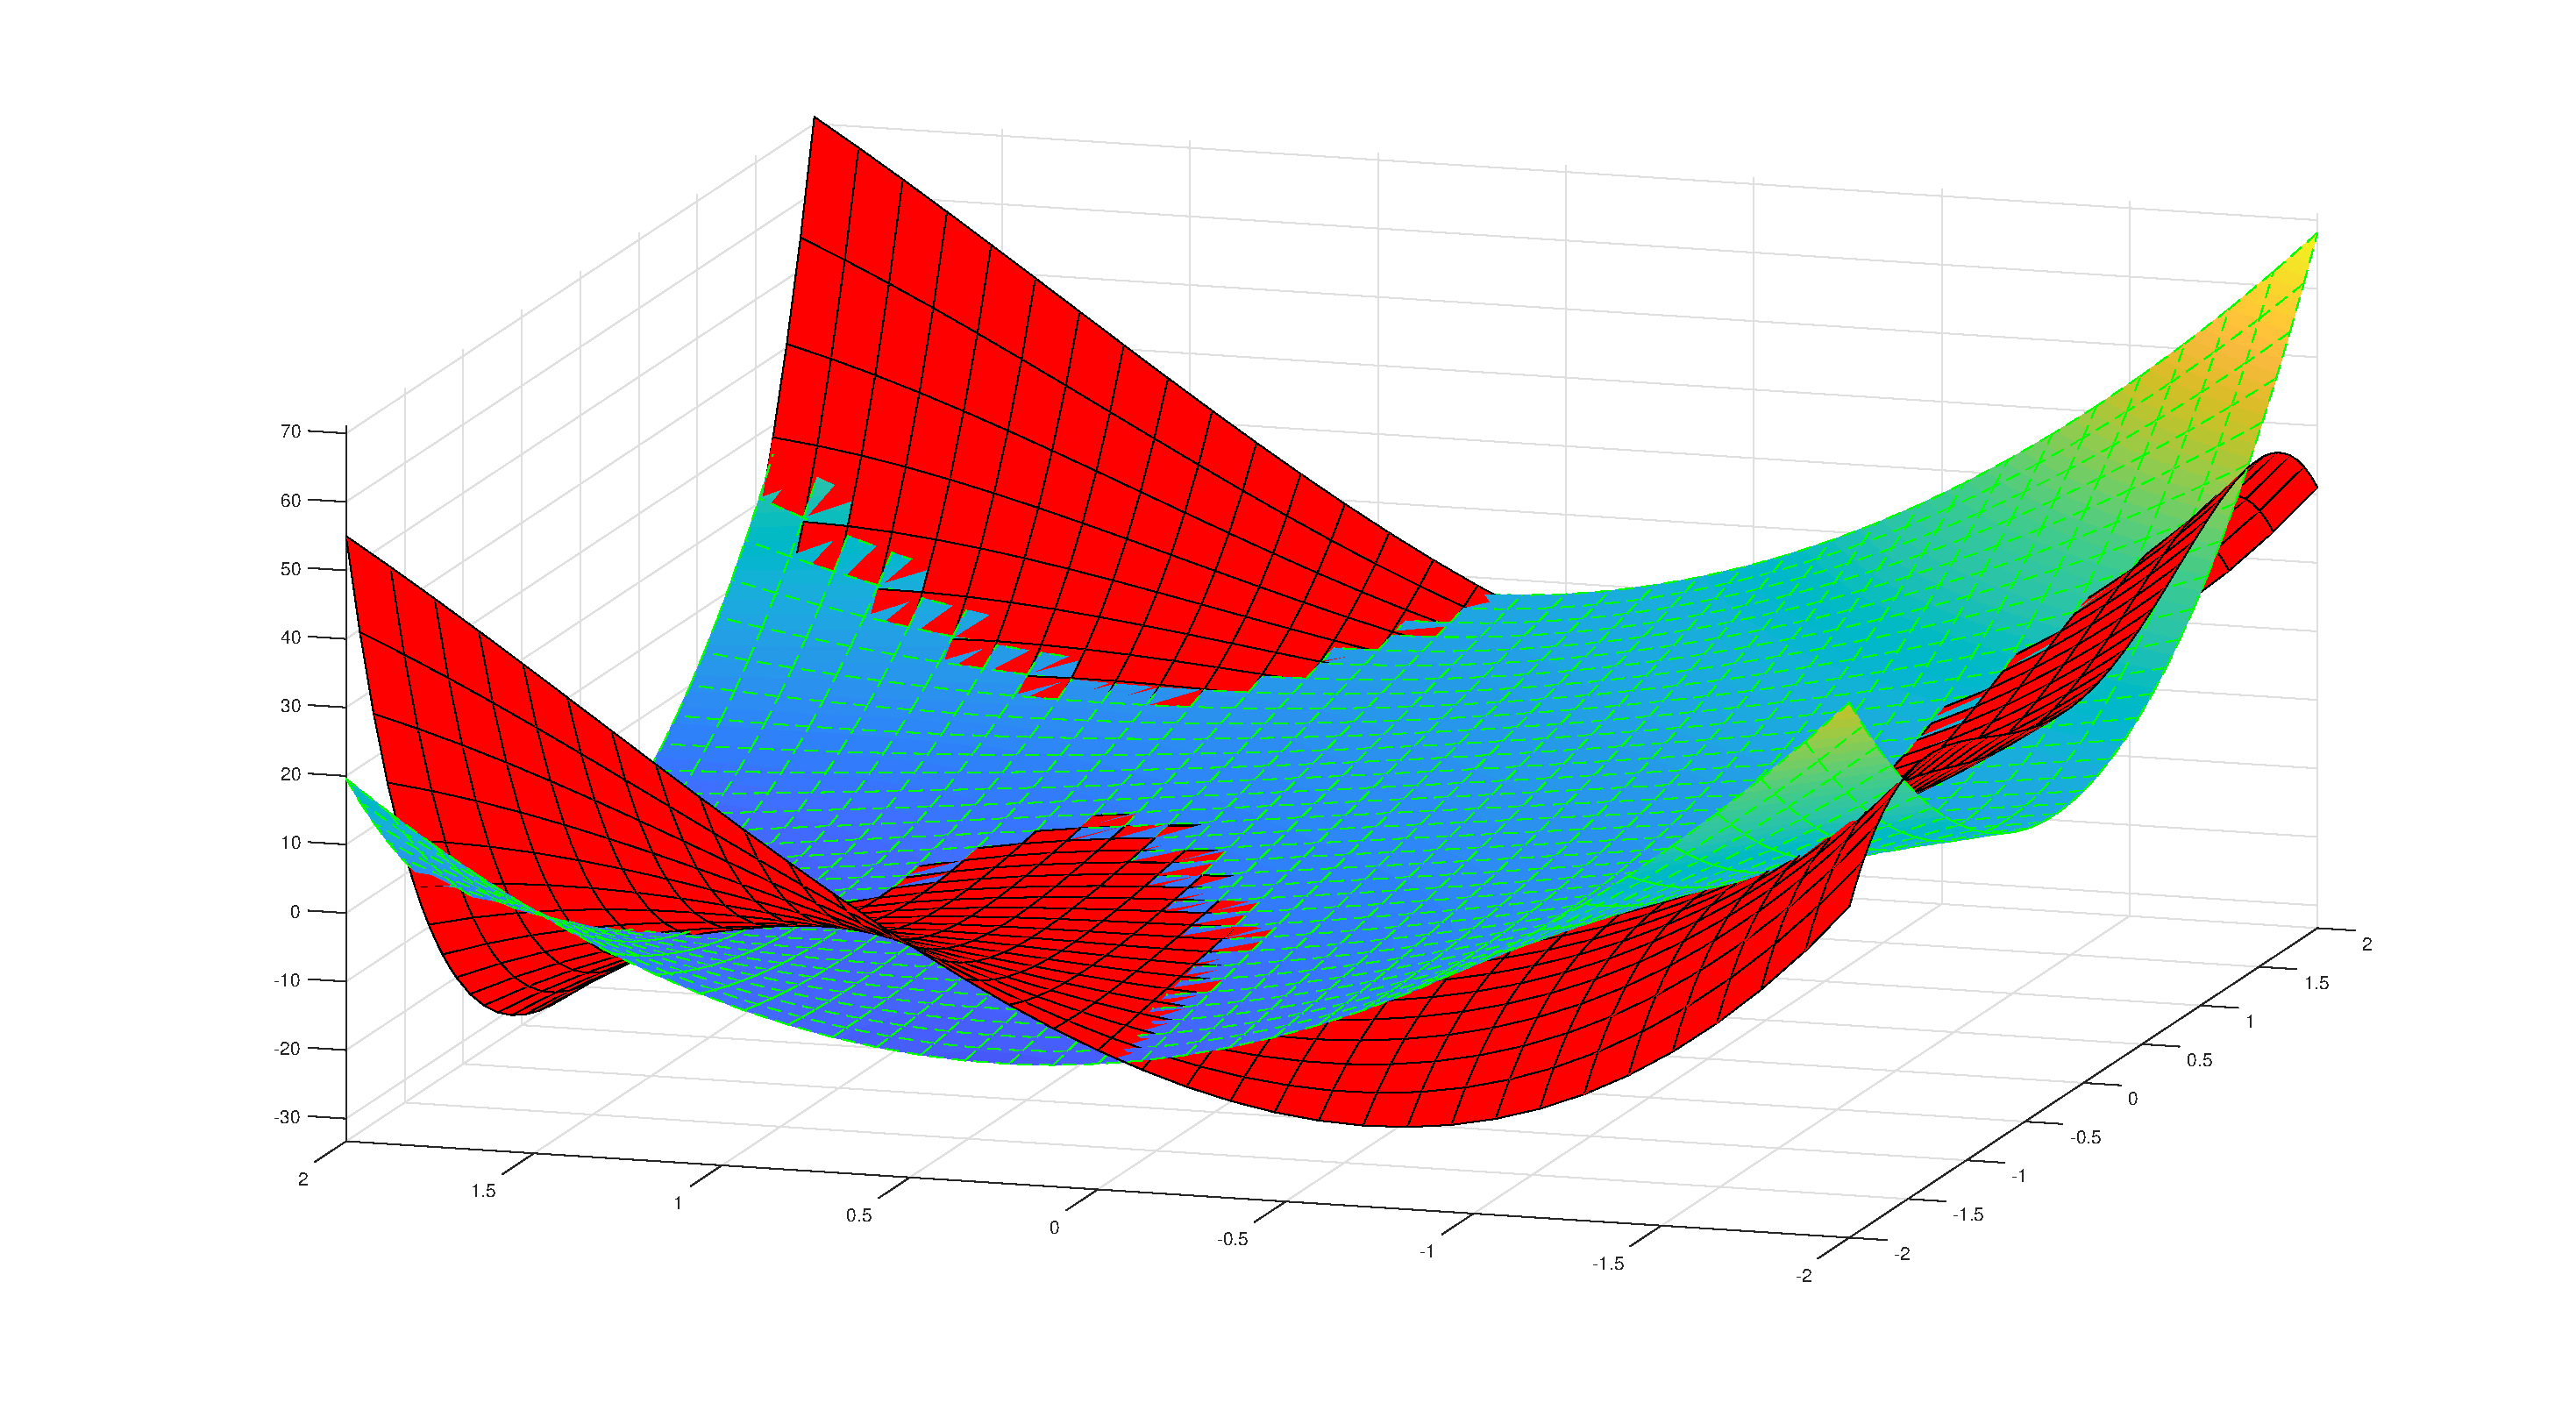
\includegraphics[width=\linewidth]{fig2.eps}
\end{figure}
Błąd średniokwadratowy wynosi $1.5181$ - funkcje z bazy nie pozwalają oddać kształtu danej funkcji, zwłaszcza gdy jej pochodna osiąga duże wartości.
\subsection{Funkcja trygonometryczna, silnie oscylująca}
\begin{lstlisting}[style=Matlab-editor]
f = @(x,y) sin(5.*(x.*x+y.*y));
presentResult(f,40,-2,2,-2,2);
\end{lstlisting}
Za pomocą danej bazy nie jest możliwe dokładnie odwzorować kształtu tego typu funkcji. Funkcja przyjmuje intuicyjnie oczekiwany kształt - przechodzi w przybliżeniu przez średnią wartość funkcji.
\begin{figure}[H]
  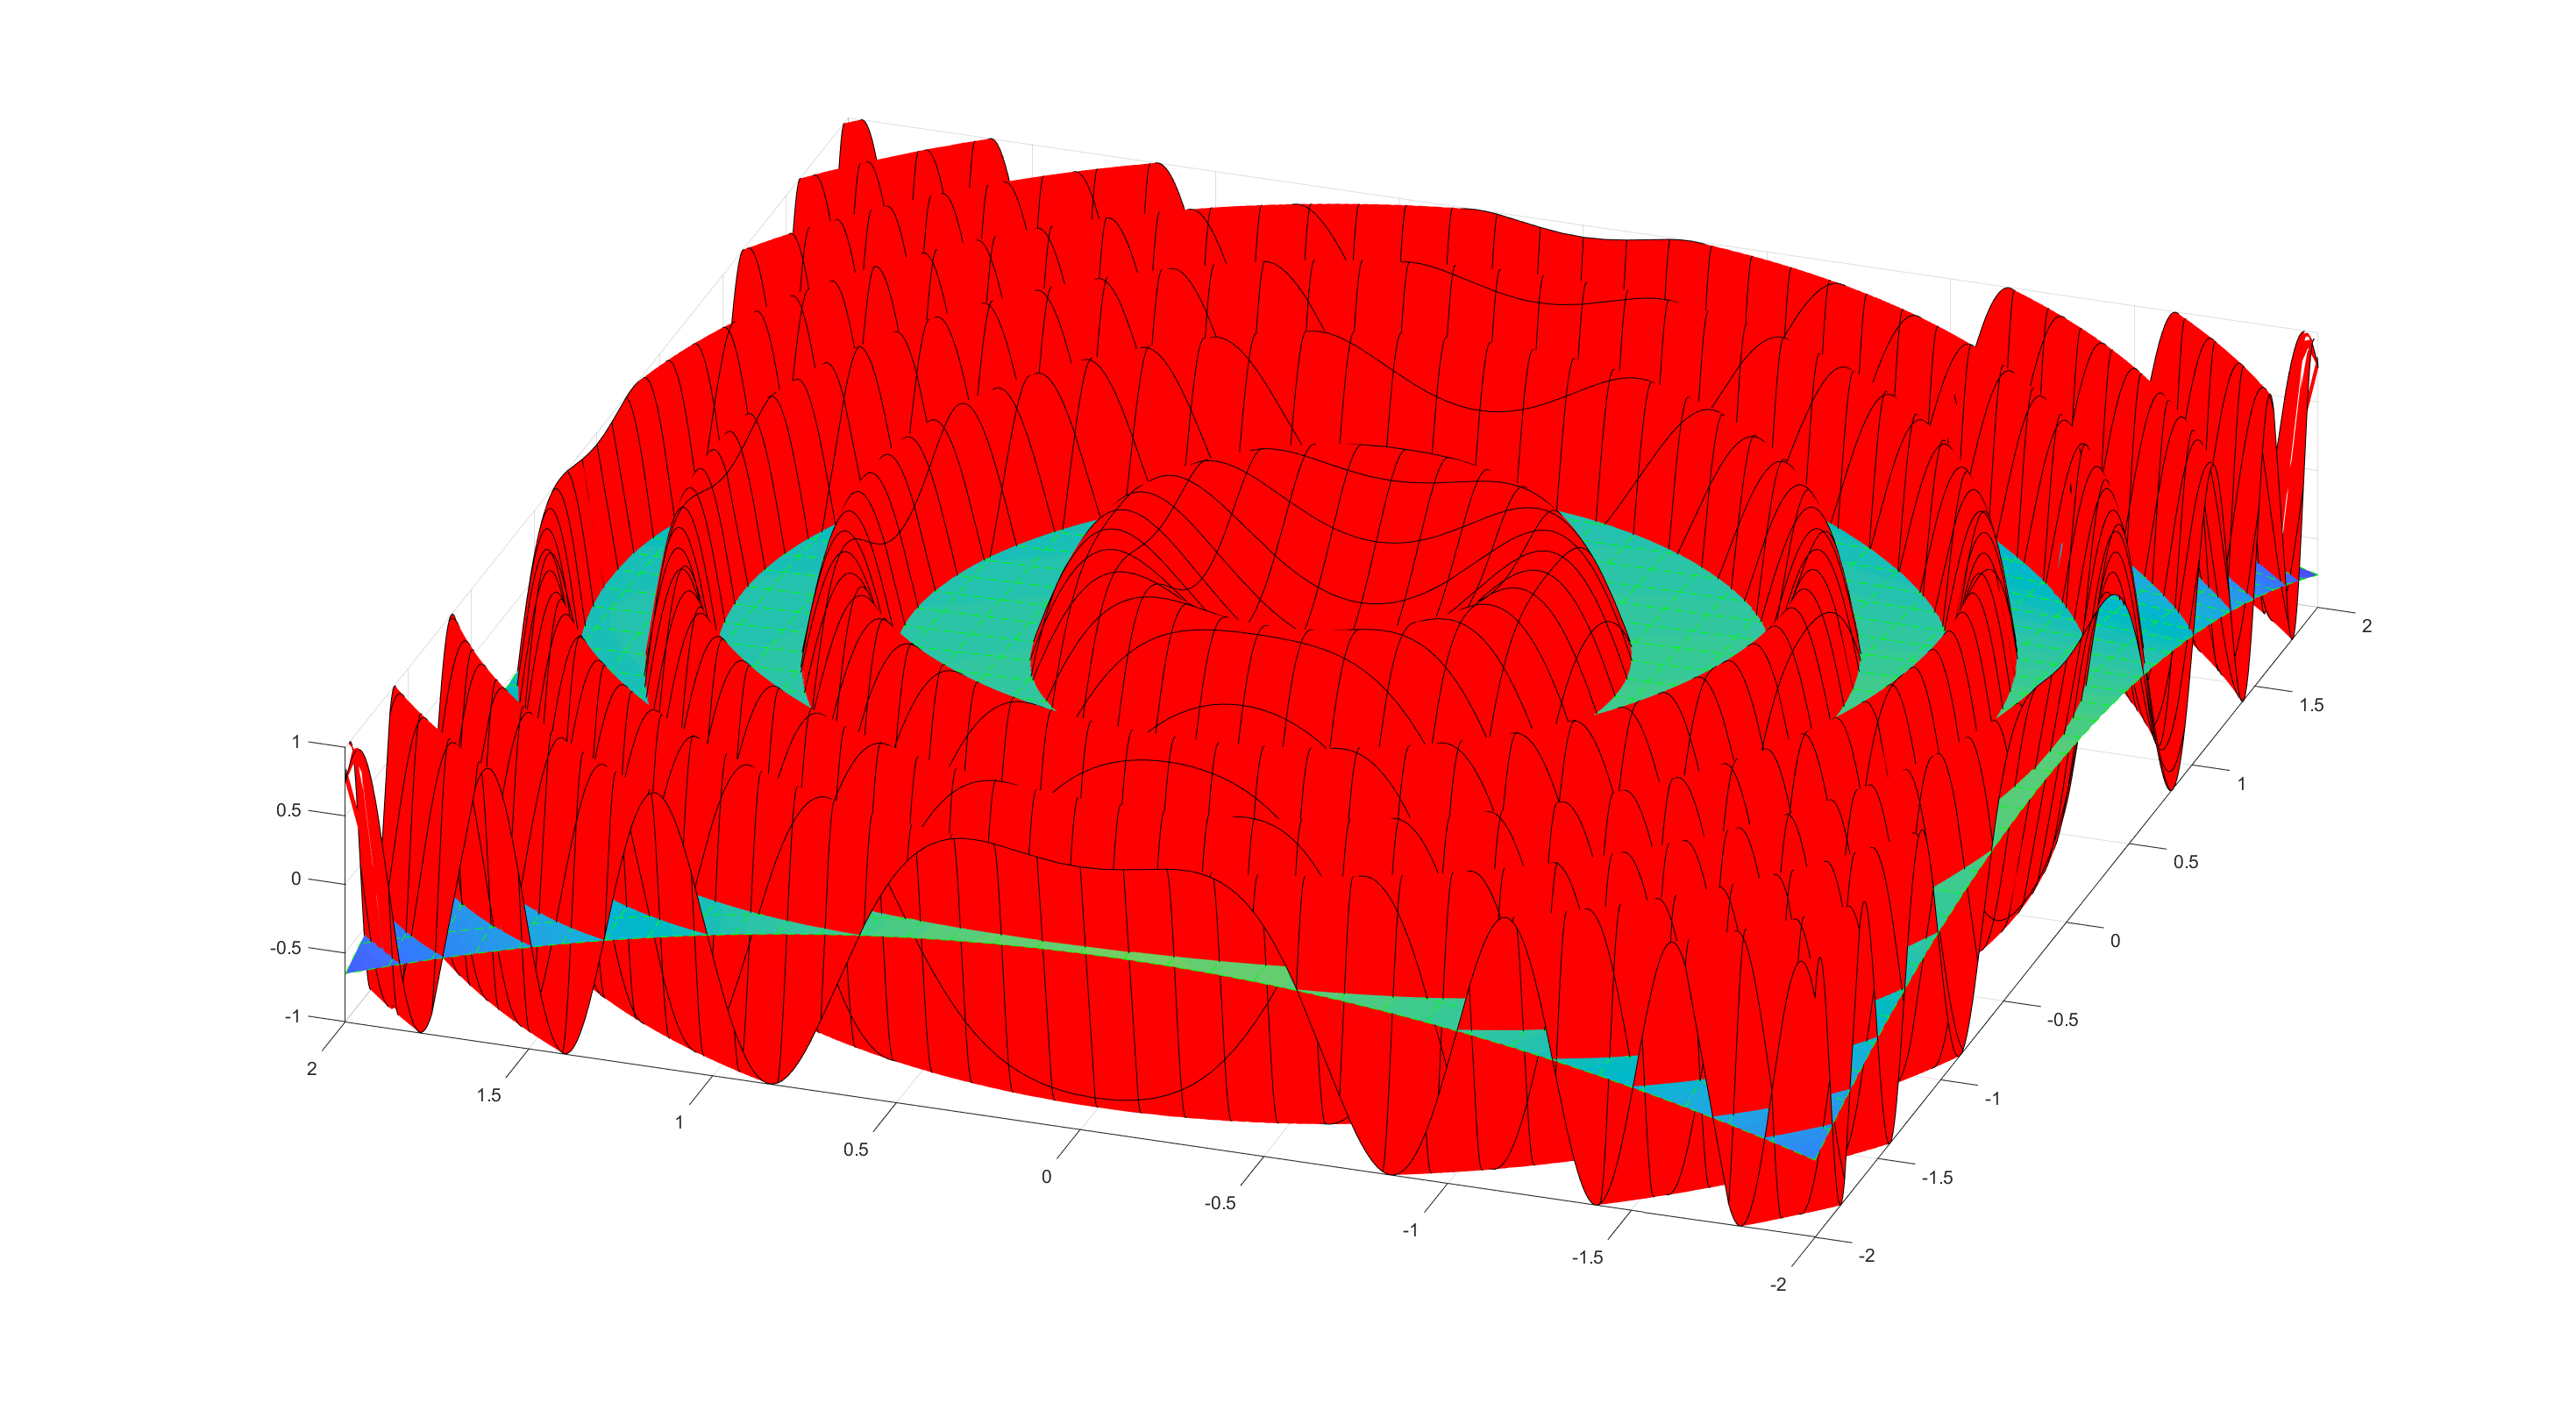
\includegraphics[width=\linewidth]{fig3.eps}
\end{figure}
Błąd średniokwadratowy w tym przypadku wynosi $0.76338$.
\subsection{Badanie wpływu ilości punktów pomiarowych na błąd średniokwadratowy}
\paragraph{}
Weźmy funkcję $f$:
\begin{lstlisting}[style=Matlab-editor]
f = @(x,y) sin(5.*(x.*x+y.*y));
\end{lstlisting}
Wykonamy poniższy skrypt i na podstawie wynikowej tabeli utworzymy wykres.
\begin{lstlisting}[style=Matlab-editor]
errors = zeros(1,1996);
for i = 4:1:2000
[~, ~, errors(i-3)] = lsfApproximation(f,i,-2,2,-2,2);
end
\end{lstlisting}
Wykres wygląda następująco:
\begin{figure}[H]
  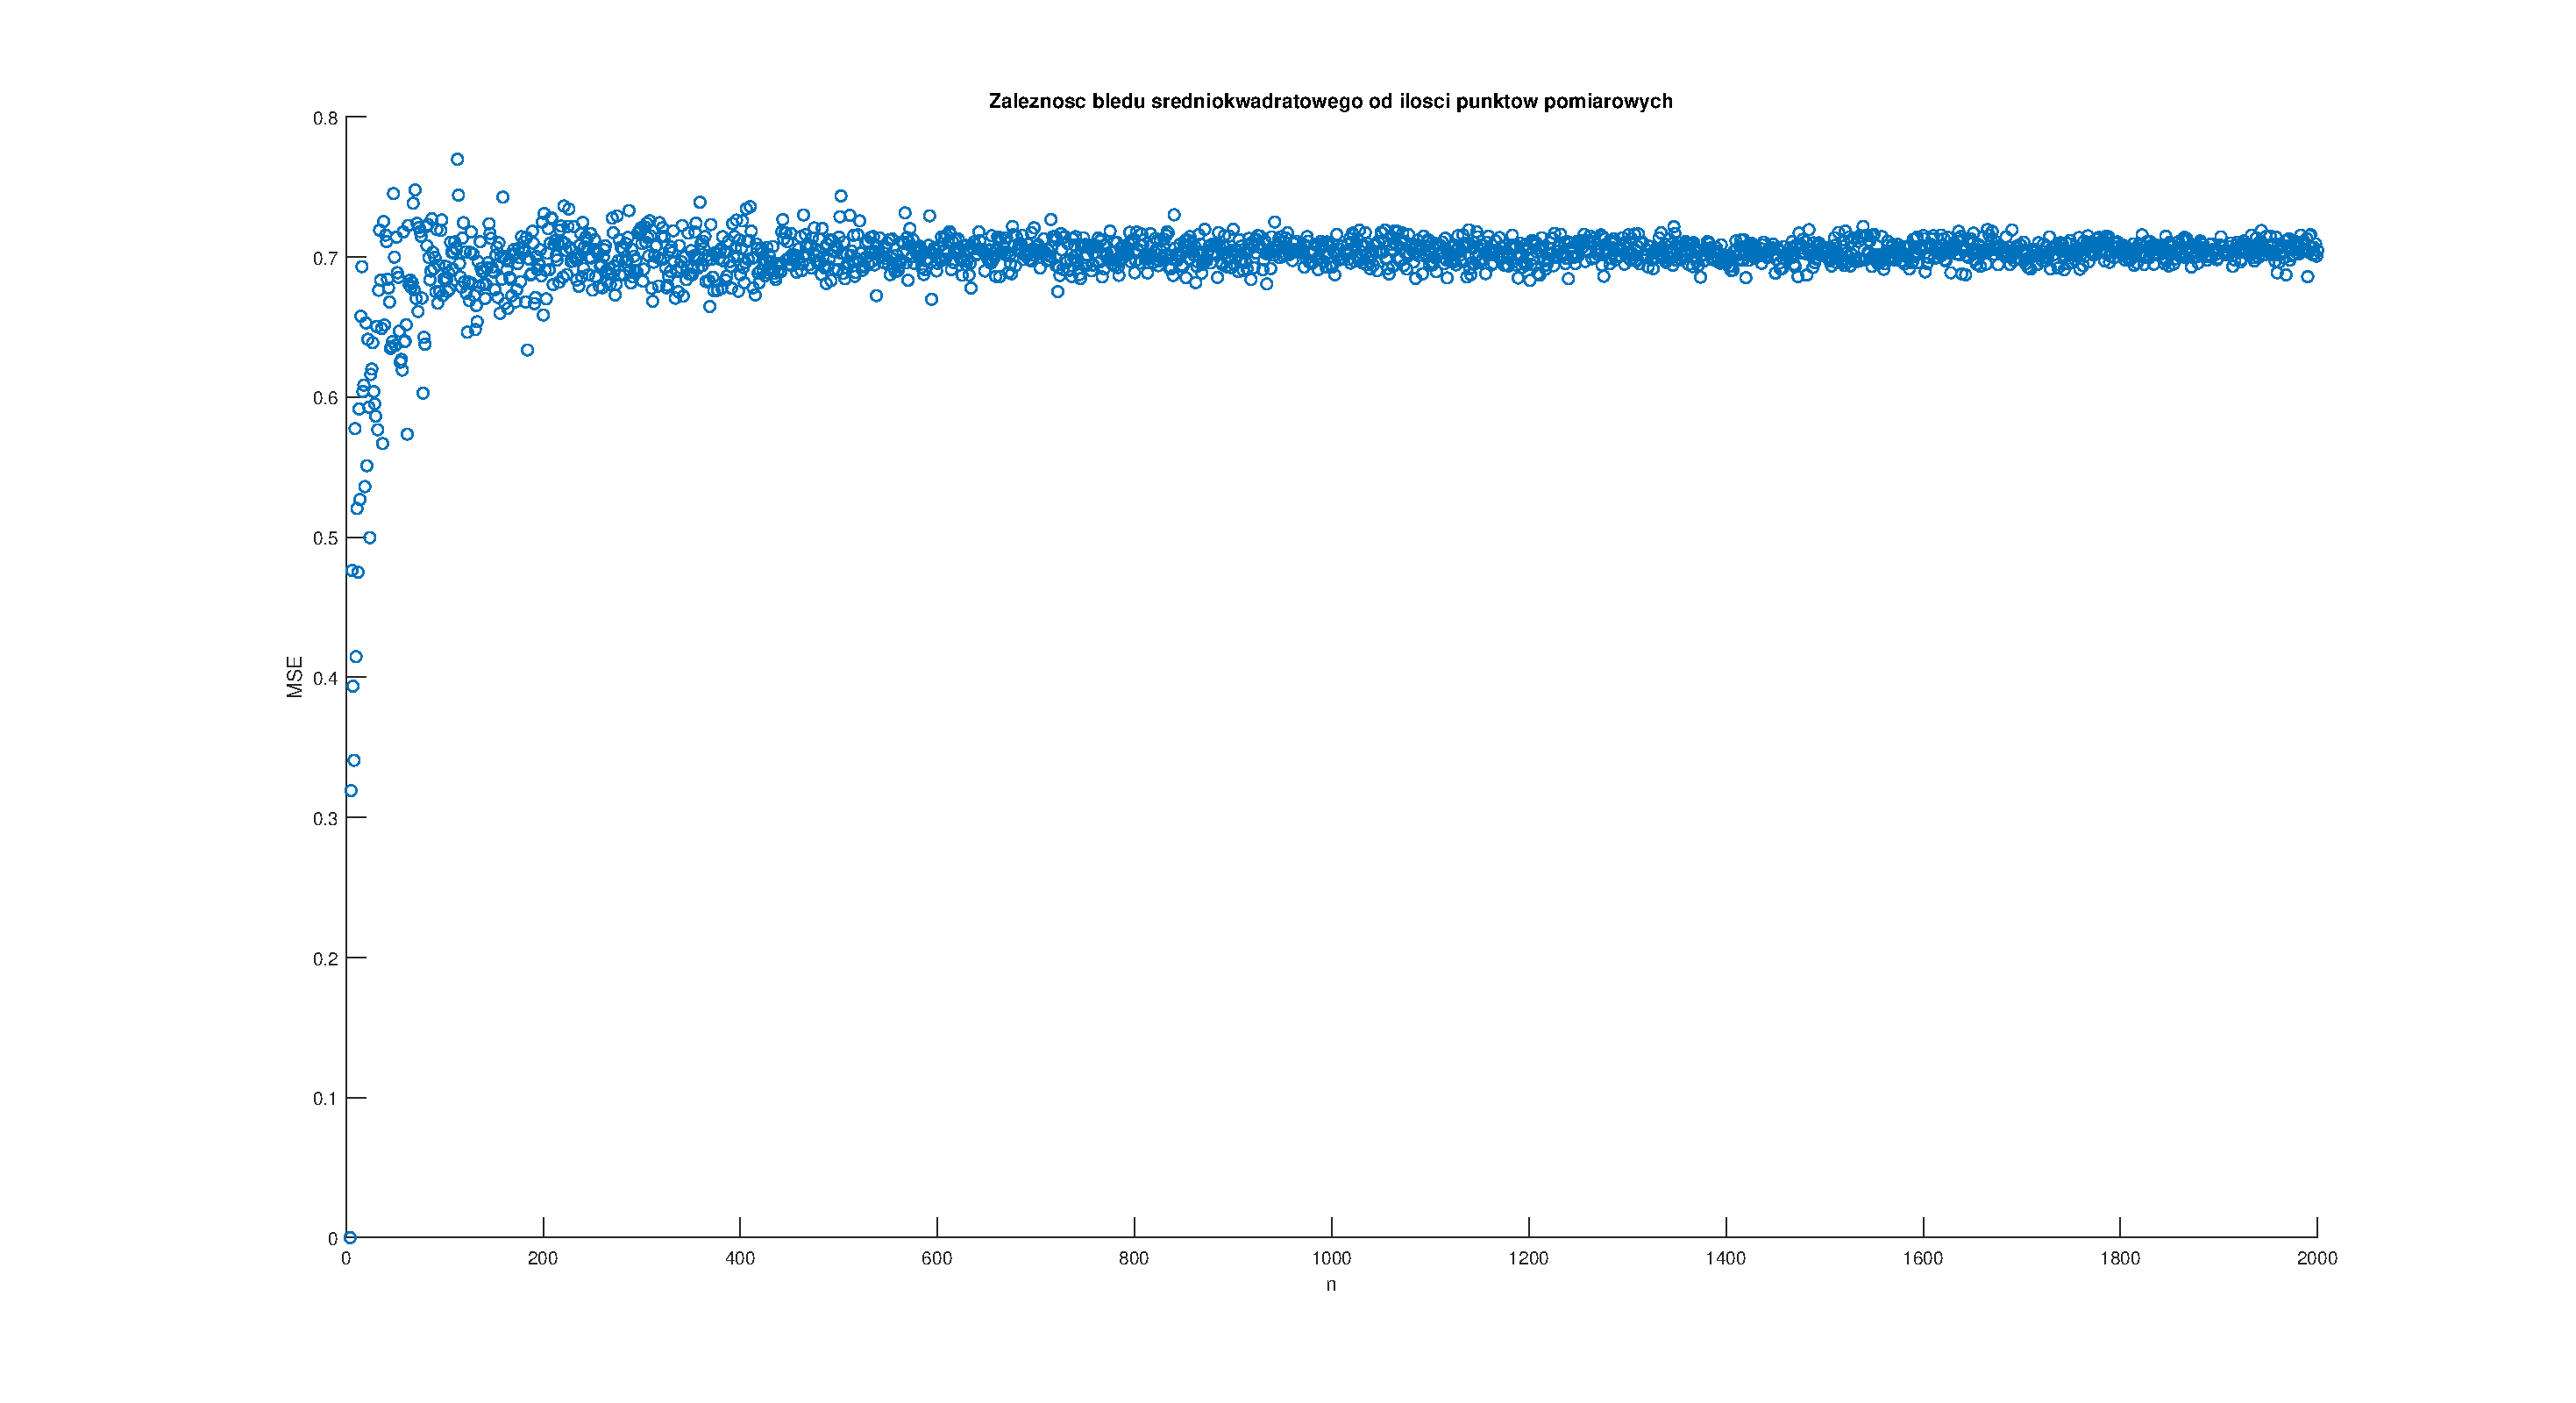
\includegraphics[width=\linewidth]{fig4.eps}
\end{figure}
Można zauważyć, że wartości błędu kwadratowego zbiegają do pewnej wartości - jest to wartość błędu dla aproksymacji średniokwadratowej ciągłej. Dla $n=4$ wartość błędu średniokwadratowego wynosi 0 - mamy wtedy faktycznie doczynienia z zadaniem interpolacji, czyli funkcja wynikowa w punktach pomiarowych przyjmuje wartości dokładne.
\subsection{Wnioski końcowe}
\begin{itemize}
\item Dokładność maszynową osiągamy tylko dla funkcji z bazy.
\item Dla złożonych funkcji nie jesteśmy w stanie oddać dokładnego kształtu za pomocą danej bazy.
\item Funkcja wynikowa przyjmuje intuicyjnie oczekiwany kształt.
\item Wraz ze wzrostem ilości punktów pomiarowych wartość błędu średniokwadratowego zbliża się do wartości błędu dla aproksymacji średniokwadratowej ciągłej.
\end{itemize}
\end{document}